\section{Proof of MSI protocol being preserving Store atomicity}
\label{safety}

In this section, we present the structure of the proof of Theorem
\fullref{storeAtomicity} for a system implementing the MSI protocol of
Figure~\ref{trans}.

We first reduce the proof of store atomicity to 4 invariants, presented in
Section \ref{firstLevel}. These invariants in turn can be reduced to 4 more
invariants presented in Section \ref{secondLevel}. The reason for choosing the 8
 invariants is because they are not specific to MSI protocol
alone; any other protocol which obeys these invariants obeys Theorem
\fullref{storeAtomicity}. We finally present the key insight which we
discovered for proving the second-level invariants in the form of 3 invariants.
We believe that these properties are common in most, if not all
invalidation-based protocols which do not perform silent drops (\ie{} protocols
in which a cache that downgrades its state informs some other cache about the
downgrade). We informally show why this is the case using the example of MESI,
MOSI and MOESI in Section \ref{mosi}.

%We use the terms write to mean handling a store request, \ie{} executing the
%StoreReq transition and read to mean handling a load request, \ie{} executing
%the LoadReq transition.

These invariants hold after any number of executions of the transactions starting
from the initial state. We use the term time $t$ to specify the global state
reached after firing $t$ transitions.

While we have proofs in Coq for each invariant our discussion will be mainly
informal for brevity. A full description can be found at~\xxx{MURALI PUT
REFERENCE HERE}.

\subsection{First level invariants}
\label{firstLevel}
Intuitively our protocol is correct because it guarantees that at most one
cache can handle a store request at a time, and that any cache that attempts to
handle a load request has the ``latest'' value. We can state this formally with
the following 4 invariants.

\begin{inv}
\textit{latestValue}:
At any time $t$, a cache $c$ which is clean for an address $a$ will have the most
up-to-date value for that address, \ie{}
\begin{enumerate}
\item $c.\data[a] = \initData(a)$ and no store request $q'$ has been processed at
any time $t'$ such that $t' < t \wedge a = q'.\addrQ$, or
\item There is a store request $q$ that was processed at time $t_q$ such that
$t_q < t \wedge a = q.\addrQ \wedge c.\data[a] = q.\dataQ$ and no other store
request $q'$ was processed at any time $t'$ such that $t_q < t' < t \wedge a =
q'.\addrQ$.
\end{enumerate}
\label{latestValue}
\end{inv}
A clean cache is defined as follows.
\begin{defn}
\textit{clean}: A cache is said to be \clean{} for an address $a$ if and only if
the state of the cache for that address is at least \Sh{} and the directory 
state for all its children is at most \Sh.
\label{clean}
\end{defn}

\begin{inv}
\textit{nonAncestorCompatible}: For two distinct caches $c_1$ and $c_2$ such
that neither is an ancestor of the other in the cache tree hierarchy (where
ancestor relation is the reflexive-transitive closure of the parent relation),
for each address $a$, $c_1.\state[a]$ and $c_2.\state[a]$ are
\textit{compatible}.
\label{nonAncestorCompatible}
\end{inv}
Compatibility of states is defined as follows.
\begin{defn}
\textit{compatibile}: Values of states $x_1$ and $x_2$ are \textit{compatible}
iff either $x_1$ or $x_2$ is \Mo{}, then the other is \In.
\label{compatible}
\end{defn}

It is easy to see that any two states $y_1 \le x_1$ and $y_2 \le x_2$ are also
compatible if $x_1, x_2$ are compatible.

\begin{inv}
\textit{processReq}: Load and store requests can be processed only at a leaf
node which is at least in the \Sh{} and \Mo{} states, respectively, for that
address.
\label{processReq}
\end{inv}

\begin{inv}
\textit{noReqAgain}:
\item For a leaf cache $c$, $c.\pos$ changes only on processing a request. In
that case, $c.\pos$ gets incremented.
\label{noReqAgain}
\end{inv}

Given these invariants, we will show how Theorem~\fullref{storeAtomicity}
follows.
%From the transitions of Figure \ref{trans}, a store may happen only
%when a leaf cache is in \Mo{} state for that
%address (Invariant~\textit{processReq}).
Leaf caches cannot be ancestors of any other node, so by Invariant
\fullref{nonAncestorCompatible}, if a leaf cache is in \Mo{} state, all other
leaf caches will be in \In{} state preventing the possibility of processing
load and store requests (because of Invariant \ref{processReq}) for the same
address at the same time at different leaf caches. This satisfies
Definition~\fullref{uniqStTimes}.

It is easy to see that Definition \fullref{uniqRespLabels}, Definition
\fullref{localOrdering} and Definition \fullref{allPrevious} directly follows
from Invariant \fullref{noReqAgain}.  As leaf caches have no children, one in
at least \Sh{} state for address $a$ is \clean{} for that address. Since
processing a load request requires the cache to be at least in the \Sh{} state,
its response, which supplies the data for that address present in the cache,
supplies the latest value by Invariant~\fullref{latestValue}. Thus, all the
conditions for Theorem~\fullref{storeAtomicity} is satisfied given Invariants
\ref{latestValue} to \ref{noReqAgain}.


\subsection{Second-level Invariants}
\label{secondLevel}

While Invariant \fullref{processReq} and \fullref{noReqAgain} can be seen
directly from the MSI transitions, correctness of Invariants
\fullref{localCompatibility1}, \fullref{localCompatibility2} and \fullref{latestValue} require further
decomposition. We present 4 more invariants for proving those two invariants.

\begin{inv}
\textit{conservative}: The state of an address in a cache is never greater than
the corresponding entry in its parent's directory.
\label{conservative}
\end{inv}

\begin{inv}
\textit{localCompatibility1}:
The state of a cache is never less than its directory entry for any of
its children.
\label{localCompatibility1}
\end{inv}
\begin{inv}
\textit{localCompatibility2}: Let $c_1$ and $c_2$ be distinct caches with the
same parent $p$. Then, $c_1.\state[a]$ and $c_2.\state[a]$ are
\textit{compatible}.
\label{localCompatibility2}
\end{inv}

\begin{inv}
\textit{noTransitWrite}: Whenever data for an address $a$ is in transit (\ie{}
$\forall t, t_s \le t \le t_r$ where $t_s$ is the time of sending the data and
$t_r$ the time of receiving the data), no cache can process a store request for
$a$, and the data must be sent from a cache which is \textit{clean}.
\label{noTransitWrite}
\end{inv}

Invariants \fullref{conservative} and \fullref{localCompatibility1} defines a
$\ge$ relation between the states of a parent and its child for any address.
Since the ancestor relation is the reflexive-transitive closure of the parent
relation, the $\ge$ relation is preserved between the states of two caches $p$
and $c$ where $p$ is the ancestor of $c$.

Any two caches $c_1, c_2$ neither of which are an ancestor of the other has a
lowest common ancestor $x$ which is an ancestor of both $c_1$ and $c_2$. $x$
has two distinct children $x_1$ and $x_2$ such that they are the ancestors of
$c_1$ and $c_2$ respectively. For any address $a$, $x_1.\state[a]$ and
$x_2.\state[a]$ are compatible by the second part of
Invariant~\fullref{localCompatibility}. It follows that $x_1.\state[a]$ and
$x_2.\state[a]$ are compatible since these values are smaller than the
respective directory values. From the previous paragraph about the relation
between the states of a cache and its ancestor, it follows that $c_1$ and $c_2$
are also compatible. This proves Invariant \fullref{nonAncestorCompatible}.

We prove Invariant \fullref{latestValue} by strong induction on time. Consider
two cases: a) cache $c$ is already \clean{} for an address $a$ at time $t$ or
b) the contrary.  If \clean{}, then it has the latest value at time $t$. Since
none of its children's directory entries can be in \Mo{}, all its descendants
should be no greater than \Sh{} for that address (because of Invariant
\fullref{conservative} and the fact that $\ge$ relation is preserved for the
state of a cache and that of its ancestor). Any non-ancestor of $c$, and
non-descendant of $c$ must be compatible (as discussed in the previous
paragraph).  Since $c$ is \clean, it is at least in the \Sh{} state, so
compatibility means that non-descendants can not be in \Mo{} state. All of
$c$'s ancestors are non-leaves, so they can not process any store request.
Therefore, no cache save $c$ may have process a store request, which means that
$c$ contains the latest value for address $a$ at time $t+1$ if it was \clean{}
at time $t$.

If $c$ was not clean at time $t$, it must have received data from either its
parent or its child. And the sender is \clean{} by Invariant
\ref{noTransitWrite}. By the induction hypothesis, it means that the sender has
the latest value for the address. Again, because of
Invariant~\ref{noTransitWrite}, no store request can be processed when the data
is in transit, which means $c$ will have the latest value for address $a$ at
time $t+1$. This establishes Invariant \fullref{latestValue}.

\subsection{Key insight for proving second-level invariants}

%ndave: This needs some repointing
We present what we believe to be the key insight for proving any cache coherence protocol.
In fact the request/response message semantics for the MSI protocol was designed to satisfy
the following three invariants.

\begin{inv}
\textit{stateChange}:
\begin{enumerate}
\item A cache downgrades its state for an address iff it sends a response for that address
\item A parent upgrades the directory entry for an address for one of its
children iff it sends a response for that child and address
\item The state or directory entry changes for an address only on sending and
receiving an response for that address, and they change to the \myto-field of the response.
\end{enumerate}
\label{stateChange}
\end{inv}

Invariant \fullref{stateChange} ensures that a response message acts as a sync
between a parent's directory entry for a child and the state of the child, as
both the sender and the receiver change their respective directory entry or
state to the \myto-field of the response.

\begin{inv}
\textit{noCross}: A response from a cache to its child for an address can not
be in transit while another response from the same child to the parent for the
same address is in transit.
\label{noCross}
\end{inv}

\begin{inv}
\textit{respFIFO}: Responses are received in the order in which they are sent,
for a source-destination pair, for the same address.
\label{respFIFO}
\end{inv}

\begin{figure}
\centering
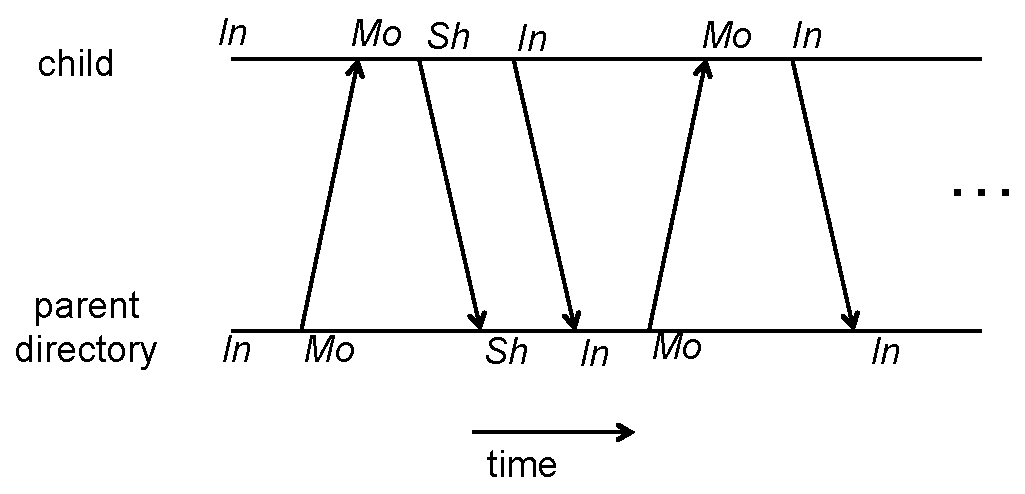
\includegraphics[scale=.5]{resps}
\caption{An example showing a sequence of responses ping ponging between a child and its parent}
\label{resps}
\end{figure}

Figure \ref{resps} shows an example of the effect of Invariants
\fullref{stateChange}, \fullref{noCross} and \fullref{respFIFO}. The directory
entry of the parent or the state of the child changes on sending and receiving
a response and the new state is showed at the points of sending or receiving
responses.
Both the cache and its parent follow the same sequence state and directory
entry changes; just that the receiver always lags slightly behind the sender.
The receiver can not send any response before receiving because of
\fullref{noCross}, thereby eliminating any scenarios where the lagging makes
reasoning complicated.

Using these three invariants (Invariant \ref{stateChange} to \ref{respFIFO}, it
is easy to see that Invariant \fullref{conservative} holds. Intuitively, going
back to Figure \ref{resps}, we can see that at all times, either there is no
response in flight, or only responses from parent in flight, or responses from
child in flight. A response from child downgrades the state and a response from
parent upgrades the directory. Since the other side simply lags behind,
Invariant \fullref{conservative} holds.

Proving the other 3 invariants in Section \ref{second-level} requires using
more properties of the MSI transistions of Figure \ref{trans}, though it is
straightforward.

%To prove Invariant \fullref{conservative} at some time $t$, consider the case
%when a child cache $c$ has sent to or received from the parent $p$ some message
%before $t$. Consider the last such message $m$ sent by or received at $c$ at
%$t'$. Let's say it is sent by $c$ at $t'$, not received. Then $p$ can not have
%received any message from $c$ after sending $m$ and before $t$ in order to not
%violate Invariant \fullref{respFIFO}.  Instead, if $c$ receives $m$ at $t'$,
%$p$ will not receive any message after sending $m$ and before $t$ in order to
%not violate Invariant \fullref{noCross}. Thus, $p$ will not receive any message
%from $c$ after sending or receiving $m$ and before $t$.  Let $t''$ be the time
%at which $p$ has sent or received $m$. Whether $p$ sends or receives $m$,
%$p.\dstate[c][a]$ at $t''+1$ will be equal to $c.\state[a]$ at $t'+1$ because
%the response messages sync up the next-state according to the transitions in
%Figure \ref{trans}. Since $p$ can not receive any message between $t''+1$ and
%$t$, it can only upgrade $p.\dstate[c][a]$. $c.\state[a]$ does not change
%between $t'+1$ and $t$ as it never changes state. Therefore, Invariant
%\fullref{conservative} holds at $t$.
%
%If no message has been sent or received by $c$ before $t$, then $p$ wouldn't
%have received any message sent by $c$ before $t$. So $p.\dstate[c][a]$ at time
%$t \ge p.\dstate[c][a]$ at time $0$ . Since the initial values of the directory
%and the child's state are both set to \In{} Invariant \textit{conservative}
%holds.
%
%To prove Invariant \fullref{localCompatibility}, it is enough to show that a
%$c.\state[a]$ is upgraded on receiving a response for $a$ from $c$'s parent $p$
%and $p.\dstate[c][a]$ is downgraded on receiving a response for $a$ from $c$.
%If this is true, then Invariant \fullref{localCompatibility} will not be
%violated on receiving a response. The transitions of Figure \ref{trans} ensures
%that Invariant \fullref{localCompatibility} is not violated when sending a
%response. Since whenever the state or directory changes, the appropriate
%response is sent or received, Invariant \fullref{localCompatibility} holds.
%
%If the value of the state of a child at the time of sending a response is the
%same as the value of the directory for that child at the parent at the time of
%receiving the response, it follows straightaway that the parent downgrades its
%directory on receiving a response from the child. This is because a child
%downgrades on sending a response and the next-states are synced on receiving
%the response.  This proof uses exactly the same arguments presented above to
%prove Invariant \fullref{conservative} -- we prove by considering the last
%message sent or received at the child before $t$ (and the case when no message
%has been sent or received). Similarly, we can show that a child upgrades its
%state on receiving a response, satisfying the conditions in the previous paragraph.
%
%Invariant \fullref{noTransitWrite} can be proved as follows. Consider a
%response sent from a parent $p$ at time $t$ received by its child $c$ at time
%$t'$. No other response can be received by the parent at time $t_p$ such that
%$t+1 \le t_p \le t'$ in order to not violate Invariant \fullref{noCross}, so
%$p.\dstate[c][a]$ at $t+1 \le p.\dstate[c][a]$ at $t'$, since the parent can
%only upgrade its directory for $c$. Similarly, no response can be sent by the
%child at time $t_c$ such that $t \le t_c \le t'$ for the same reason and hence
%$c.\state[a]$ at $t \le c.\state[a]$ at $t'$ since the child can only downgrade
%its state.  This means that during $t_p$ such that $t+1 \le t_p \le t'$,
%$p.\dstate[c][a] > \In$ and (hence $p.\state[a] > \In$ by the first part of
%Invariant \fullref{localCompatibility}) since the parent upgraded its directory
%for $c$ at $t$.  Similarly, during $t_c$ such that $t \le t_c \le t'$,
%$c.\state[a] < \Mo$ since the child upgrades its state at $t'$. We have already
%shown that (in the proof of Invariant \fullref{latestValue}) if any cache is
%not in \In{} state, no non-descendent cache can process a store request. In
%this case, during the times between $t$ and $t'$, $p$ is not in \In{} state.
%Among $p$'s directory entries, all of them save the entry for $c$ is not in
%\Mo{} state, so none of the descendents of $p$'s children, save $c$'s
%descendents can process a store request. During the times between $t$ and $t'$,
%$c$'s state is $< \Mo{}$, so neither $c$ nor its descendents can process a store
%request, proving Invariant \fullref{noTransitWrite}.

%from the parent and child respectively, it is sufficient to show that the previous state
%or the 
%
%Invariant~\textit{conservative} can be proved by
%further breaking them into the following invariants between a parent-child pair
%of caches.
%
%\begin{inv}
%\textit{stateChange}:
%\begin{enumerate}
%\item A child sends a response to its parent iff it downgrades its state.
%\item A parent sends a response to a child iff it upgrades the directory of
%that child.
%\item The state and the directory can change only on sending and receiving a
%response; the receiving entity changes its value to that of the sending entity
%immediately after sending the response message.
%\end{enumerate}
%\label{stateChange}
%\end{inv}
%
%\begin{inv}
%\textit{respFIFO}: Responses are received in the order in which they are sent,
%for a source-destination pair, for the same address.
%\label{respFIFO}
%\end{inv}
%
%\begin{inv}
%\textit{noCross}: A response from a cache to its child for an address can not
%be in transit while another response from the same child to the parent for the
%same address is in transit.
%\label{noCross}
%\end{inv}
%
%Invariant~\textit{conservative} at any time $t$ for child cache $c$ and parent
%$p$ for an address $a$ can be proved as follows. Consider the case when
%$c.\state[a]$ never changed before $t$, then $c.\state[a] = \In$ because of the
%initialization conditions described in Section \ref{System}. No response would
%have been sent by $c$ to its parent for address $a$ before $t$, otherwise
%$c.\state[a]$ would have changed. Thus the parent would not have received any
%response from $c$, $p.\dstate[c][a]$ could have changed only by sending a
%response to $c$ which can only upgrade it from the initial value of $\In$. Thus
%at $t$, $p.\dstate[c][a] \ge c.state[a]$.
%
%Now consider the case when $c.\state[a]$ last changed at $t'$ such that $t' <
%t$ because of receiving a response from $p$, sent at $t''$. $c.\state[a]$ at
%$t'+1 = p.\dstate[c][a]$ at $t''+1$ because of Invariant \fullref{stateChange}.
%$c$ neiter sends nor receives a response at any $t_i$ such that $t' < t_i < t$.
%If $p$ received a response at some $t_m$ such that $t'' < t_m < t$,
%then it would either violate Invariant \fullref{noCross}, or the fact that no
%message was sent between $t' < t_i < t$ from $c$. Thus, $p.\dstate[c][a]$ at $t
%\ge p.\dstate[c][a]$ at $t''+1$ because any message sent can only upgrade
%$p.\dstate[a]$. This ensures that Invariant \fullref{conservative} is obeyed. We
%can similarly prove this invariant holds when $c.\state[a]$ last changes before
%$t$ by sending a response.
%
%Invariant \fullref{stateChange} can be proved directly from the atomic
%transitions for MSI. Other protocols have similar atomic transitions obeying
%these invariants.
%
%Invariant \fullref{respFIFO} can be enforced by the interconnect network which
%ensures a FIFO ordering for messages sent between a pair of nodes.
%
%---------------------------------------------
%
%%Invariant \fullref{respFIFO} is known as point-to-point FIFO ordering in the
%%Network-on-Chip NoC community, and is enforced by common routing algorithms
%%like Dimension-ordered routing \cite{dimension}. Only the parent-to-child
%%channels need to be FIFO ordered, the FIFO ordering in child-to-parent channels
%%can be enforced using the protocol itself.
%
%\begin{inv}
%\textit{noTransitEqual}: When no response is in transit for an address, then
%the state of a cache for that address is the same as its parent's directory for
%that cache and address.
%\label{noTransitEqual}
%\end{inv}
%
%Proving Invariants \fullref{inTransitCondition} and \textit{noTransitEqual},
%needs two further invariants, along with Invariant \fullref{stateChange}.
%
%Invariant \fullref{inTransitCondition} can be proved as follows. Whenever a
%response from a child to the parent is in transit, the parent can not send any
%response to the child, or it will violate Invariant \fullref{noCross}. Using the fact that 
%
%
%
%
%
%
%
%\begin{inv}
%\textit{inTransitCondition}:
%\begin{enumerate}
%\item When a response is sent from a child $c$ at time $t$ for an address $a$,
%and has not been received by the parent $p$ before time $t'$, $\forall t_i, t <
%t_i \le t' @-> c.\state[a]$ at $t_i \le c.\state[a]$ at $t+1$ and $\forall t_i,
%t \le t_i \le t' @->$ $p.\dstate[c][a]$ at $t_i \ge c.\state[a]$ at $t$.
%\item When a response is sent from parent $p$ at time $t$ for an address $a$,
%and has not been received by its child $c$ before time $t'$, $\forall t_i, t <
%t_i \le t' @-> p.\dstate[c][a]$ at $t_i \ge p.\dstate[c][a]$ at $t+1$ and
%$\forall t_i, t \le t_i \le t' @->$ $c.\state[a]$ at $t_i \le p.\dstate[c][a]$ at
%$t$.
%\end{enumerate}
%\label{inTransitCondition}
%\end{inv}
%
%\begin{inv}
%\textit{prevState}: When a response is received from a child to the parent
%(parent to child) for an address, the state of the child for that address at
%the time of sending (receiving) the response is the same as the parent's
%directory for that child and address at the time of receiving (sending) the
%response.
%\label{prevState}
%\end{inv}
%
%
%
%%Top
%%a) conservative: forall p c a t, parent c p -> dir p c a t >= state c a t
%%b) forall p c a t, parent c p -> state p a t >= dir p c a t
%%c) forall c1 c2 a t, sibling c1 c2 -> compatible c1 c2 a t
%%d) nextClean: ~ clean c a t -> clean c a (S t) -> exists s d ts, recv data s a t d /\ send data s a ts d /\ clean s a ts /\ ts <= t /\ forall ti, ts <= ti < t ->  ~ write a ti
%%
%%(from=state(t1)=dir(t2) -> betweenPSendCRecv:dir(t)>=to&state(t)<=from, betweenCSendPRecv:state(t)<=to&dir(t)>=from), noMesgImp:state(t)=dir(t) -> conservative (ignore from=, use only a, b)
%%a) Child sends message iff it downgrades
%%b) Parent sends message iff it upgrades
%%c) State is changed only on sending or receiving a message
%%d) FIFO messages
%%e) cross: Message from child and parent do not cross
%%
%%cross:
%%a) parent send message only on receiving request
%%b) req from child does not overtake response from child (prove using the from states)
%%c) resp from parent does not overtake request from parent
%%d) voluntary response sent from child only when not waiting
%%
%%In this section we specify a set of important invariants for a parent-child pair of caches.

%%  LocalWords:  Invariants invariants
